\begin{figure}[H]
	\centering
	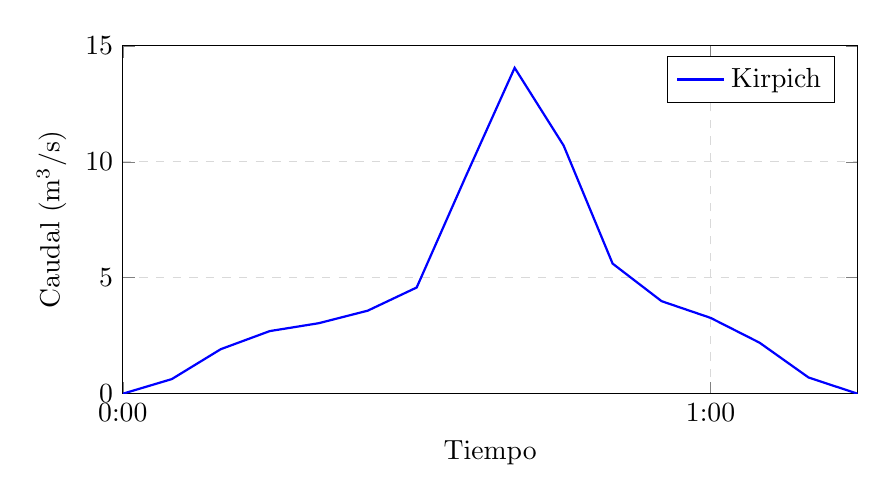
\begin{tikzpicture}
		\begin{axis}[
			width=0.9\textwidth,
			height=6cm,
			xlabel={Tiempo},
			ylabel={Caudal (m$^3$/s)},
			xmin=0,
			xmax=75,
			ymin=0,
			ymax=15,
			grid=major,
			grid style={dashed, gray!30},
			legend pos=north east,
			xtick={0, 60},
			xticklabels={0:00, 1:00},
			]
		% Kirpich
		\addplot [
		blue,
		thick,
		solid,
		] coordinates {
				(0, 0.00) (5, 0.63) (10, 1.92) (15, 2.70) (20, 3.04)
				(25, 3.58) (30, 4.58) (35, 9.36) (40, 14.05) (45, 10.70)
				(50, 5.61) (55, 3.99) (60, 3.27) (65, 2.20) (70, 0.70)
				(75, 0.00)
		};
		\addlegendentry{Kirpich}

		\end{axis}
	\end{tikzpicture}
	\caption{Hidrograma - Kirpich + BLOCKS $T_r$=10 años ($Q_p$=14.047 m$^3$/s)}
	\label{fig:hydro_kirpich_blocks_Tr10}
\end{figure}
